%package list
\documentclass{article}
\usepackage[top=3cm, bottom=3cm, outer=3cm, inner=3cm]{geometry}
\usepackage{multicol}
\usepackage{graphicx}
\usepackage{url}
%\usepackage{cite}
\usepackage{hyperref}
\usepackage{array}
%\usepackage{multicol}
\newcolumntype{x}[1]{>{\centering\arraybackslash\hspace{0pt}}p{#1}}
\usepackage{natbib}
\usepackage{pdfpages}
\usepackage{multirow}
\usepackage[normalem]{ulem}
\useunder{\uline}{\ul}{}
\usepackage{svg}
\usepackage{xcolor}
\usepackage{listings}
\lstdefinestyle{ascii-tree}{
    literate={├}{|}1 {─}{--}1 {└}{+}1 
  }
\lstset{basicstyle=\ttfamily,
  showstringspaces=false,
  commentstyle=\color{red},
  keywordstyle=\color{blue}
}
%\usepackage{booktabs}
\usepackage{caption}
\usepackage{subcaption}
\usepackage{float}
\usepackage{array}

\newcolumntype{M}[1]{>{\centering\arraybackslash}m{#1}}
\newcolumntype{N}{@{}m{0pt}@{}}


%%%%%%%%%%%%%%%%%%%%%%%%%%%%%%%%%%%%%%%%%%%%%%%%%%%%%%%%%%%%%%%%%%%%%%%%%%%%
%CREACIÓN DE VARIABLE
\newcommand{\itemStudent}{- Gordillo Mendoza Jose\newline - Lopez Arela Ower\newline - Condori Pinto Juan Jose\newline - Borda Espinoza Gabriela Nayely}
\newcommand{\itemCourse}{Estructura de Datos y Algoritmos}
\newcommand{\itemCourseCode}{20222083}
\newcommand{\itemSemester}{III}
\newcommand{\itemUniversity}{Universidad Nacional de San Agustín de Arequipa}
\newcommand{\itemFaculty}{Facultad de Ingeniería de Producción y Servicios}
\newcommand{\itemDepartment}{Departamento Académico de Ingeniería de Sistemas e Informática}
\newcommand{\itemSchool}{Escuela Profesional de Ingeniería de Sistemas}


%AQUIIII: CAMBIA LA INFO DEL LAB
\newcommand{\itemAcademic}{2023 - A}
\newcommand{\itemInput}{Del 23 Junio 2023}
\newcommand{\itemOutput}{Al 30 Junio 2023}
\newcommand{\itemPracticeNumber}{05}
\newcommand{\itemTheme}{Arbol AVL}
%%%%%%%%%%%%%%%%%%%%%%%%%%%%%%%%%%%%%%%%%%%%%%%%%%%%%%%%%%%%%%%%%%%%%%%%%%%%


%PARA EL PIE DE PÁGINA
\usepackage{fancyhdr}
\pagestyle{fancy}
\fancyhf{}
\setlength{\headheight}{30pt}
\renewcommand{\headrulewidth}{1pt}
\renewcommand{\footrulewidth}{1pt}
\fancyhead[L]{\raisebox{-0.2\height}{
\includegraphics[width=3cm]{img/logo_episunsa.png}}}
\fancyhead[C]{\fontsize{7}{7}\selectfont	\itemUniversity \\ \itemFaculty \\ \itemDepartment \\ \itemSchool \\ \textbf{\itemCourse}}
\fancyhead[R]{\raisebox{-0.2\height}{
\includegraphics[width=1.2cm]{img/logo_abet}}}
\fancyfoot[L]{Grupo 04}
\fancyfoot[C]{\itemCourse}
\fancyfoot[R]{Página \thepage}

% para el codigo fuente
\usepackage{listings}
\usepackage{color, colortbl}
\definecolor{dkgreen}{rgb}{0,0.6,0}
\definecolor{gray}{rgb}{0.5,0.5,0.5}
\definecolor{mauve}{rgb}{0.58,0,0.82}
\definecolor{codebackground}{rgb}{0.95, 0.95, 0.92}
\definecolor{tablebackground}{rgb}{0.8, 0, 0}

\lstset{frame=tb,
	language=bash,
	aboveskip=3mm,
	belowskip=3mm,
	showstringspaces=false,
	columns=flexible,
	basicstyle={\small\ttfamily},
	numbers=none,
	numberstyle=\tiny\color{gray},
	keywordstyle=\color{blue},
	commentstyle=\color{dkgreen},
	stringstyle=\color{mauve},
	breaklines=true,
	breakatwhitespace=true,
	tabsize=3,
	backgroundcolor= \color{codebackground},
}


\begin{document}
	%CARÁTULA
	\vspace*{10px}
	
	\begin{center}	
		\fontsize{17}{17} \textbf{ Informe de Laboratorio \itemPracticeNumber}
	\end{center}
	\centerline{\textbf{\Large Tema: \itemTheme}}
	%\vspace*{0.5cm}	

	\begin{flushright}
		\begin{tabular}{|M{2.5cm}|N|}
			\hline 
			\rowcolor{tablebackground}
			\color{white} \textbf{Nota}  \\
			\hline 
			     \\[30pt]
			\hline 			
		\end{tabular}
	\end{flushright}	

	\begin{table}[H]
		\begin{tabular}{|x{4.7cm}|x{4.8cm}|x{4.8cm}|}
			\hline 
			\rowcolor{tablebackground}
			\color{white} \textbf{Estudiante} & \color{white}\textbf{Escuela}  & \color{white}\textbf{Asignatura}   \\
			\hline 
			{\itemStudent \par \itemEmail} & \itemSchool & {\itemCourse \par Semestre: \itemSemester \par Código: \itemCourseCode}     \\
			\hline 			
		\end{tabular}
	\end{table}		
	
	\begin{table}[H]
		\begin{tabular}{|x{4.7cm}|x{4.8cm}|x{4.8cm}|}
			\hline 
			\rowcolor{tablebackground}
			\color{white}\textbf{Laboratorio} & \color{white}\textbf{Tema}  & \color{white}\textbf{Duración}   \\
			\hline 
			\itemPracticeNumber & \itemTheme & 04 horas   \\
			\hline 
		\end{tabular}
	\end{table}
	
	\begin{table}[H]
		\begin{tabular}{|x{4.7cm}|x{4.8cm}|x{4.8cm}|}
			\hline 
			\rowcolor{tablebackground}
			\color{white}\textbf{Semestre académico} & \color{white}\textbf{Fecha de inicio}  & \color{white}\textbf{Fecha de entrega}   \\
			\hline 
			\itemAcademic & \itemInput &  \itemOutput  \\
			\hline 
		\end{tabular}
	\end{table}

    %INFORME
    \section{Tarea}
    \begin{itemize}
        \item Elabore un informe implementando Arboles AVL con toda la lista de operaciones  search(), getMin(), getMax(), parent(), son(), insert(), remove().
        \item INPUT: Una sola palabra en mayusculas.
        \item OUTPUT: Se debe contruir el ´arbol AVL considerando el valor decimal de su codigo ascii.
        \item Luego, pruebe todas sus operaciones implementadas.
        \item Estudie la librerıa Graph Stream para obtener una salida grafica de su implementacion.
        \item Utilice todas las recomendaciones dadas por el docente.
    \end{itemize}
    \section{GitHub}
    \begin{itemize}	
        \item \url{https://github.com/jcondoripin/Eda_Labs/tree/main/Lab05}	

\end{itemize}
\clearpage
\section{Resolucion}

    \begin{itemize}
        \item Class \textbf{NodoAVL.java}
    \end{itemize}
    \begin{lstlisting}[caption={\textbf{Parte 1: Declaración de variables y constructores}}]
        \begin{lstlisting}[language=bash][H] 
            private T valor;
            private NodoAVL<T> left;
            private NodoAVL<T> right;
            private int bf;
            public NodoAVL(T value, NodoAVL<T> left, NodoAVL<T> right) {
                this.left = left;
                this.right = right;
                this.valor = value;
                this.bf = 0;
            }
            public NodoAVL(T value) {
                this(value, null, null);
            }
         \end{lstlisting}
En esta parte, se declaran las variables valor, left, right y bf. valor es de tipo genérico T y representa el valor almacenado en el nodo. left y right son referencias a los hijos izquierdo y derecho del nodo, respectivamente. bf representa el factor de equilibrio del nodo, que es la diferencia entre las alturas de los subárboles derecho e izquierdo.

Se definen dos constructores. El primer constructor toma un valor, un nodo hijo izquierdo y un nodo hijo derecho, y establece los valores correspondientes en el nodo actual. El segundo constructor toma solo un valor y establece los hijos izquierdo y derecho como nulos.

 \begin{lstlisting}[caption={\textbf{Parte 2: Métodos de acceso y modificación}}]
        \begin{lstlisting}[language=bash][H] 
            public void setRight(NodoAVL<T> right) {
                this.right = right;
            }
            public void setLeft(NodoAVL<T> left) {
                this.left = left;
            }
            public NodoAVL<T> getRight() {
                return this.right;
            }
            public NodoAVL<T> getLeft() {
                return this.left;
            }
            public void setValue(T value) {
                this.valor = value;
            }
            public T getValue() {
                return this.valor;
            }
            public void setBf(int alt) {
                this.bf = alt;
            }
            public int getBf() {
                return this.bf;
            }
         \end{lstlisting}
Estos métodos proporcionan acceso y modificación a los diferentes campos del nodo: Los métodos setRight y setLeft se utilizan para establecer los hijos derecho e izquierdo del nodo. Los métodos getRight y getLeft se utilizan para obtener los hijos derecho e izquierdo del nodo. Los métodos setValue y getValue se utilizan para establecer y obtener el valor almacenado en el nodo. Los métodos setBf y getBf se utilizan para establecer y obtener el factor de equilibrio del nodo.


    \begin{itemize}
        \item Class \textbf{ItemDuplicated.java}
    \end{itemize}
    \begin{lstlisting}[caption={\textbf{Se puede lanzar cuando se encuentra un elemento duplicado en algún contexto específico.}}]
        \begin{lstlisting}[language=bash][H] 
            package Lab05.Exceptions;
            
            public class ItemDuplicated extends Exception {
                public ItemDuplicated(String s){
                    super(s);
                }
            }
         \end{lstlisting}
La clase ItemDuplicated define una excepción personalizada que se lanza cuando se encuentra un elemento duplicado en un contexto específico. Permite manejar y notificar de manera explícita la presencia de duplicados.


\begin{itemize}
        \item Class \textbf{NotFoundException.java}
    \end{itemize}
    \begin{lstlisting}[caption={\textbf{Excepción personalizada llamada "NotFoundException"}}]
        \begin{lstlisting}[language=bash][H] 
            package Lab05.Exceptions;
            
            public class NotFoundException extends Exception {
                public NotFoundException(String s) {
                    super(s);
                }
            }
         \end{lstlisting}
La clase NotFoundException es una excepción personalizada que se lanza cuando no se encuentra un elemento en un contexto específico.


\begin{itemize}
        \item Class \textbf{AVLTree.java}
    \end{itemize}
    \begin{lstlisting}[caption={\textbf{Árbol de Búsqueda y Equilibrio de Altura}}]
            package Lab05;
            
            import Lab05.Exceptions.NotFoundException;
            import Lab05.Exceptions.ItemDuplicated;
            
            public class AVLTree<T extends Comparable<T>> {
                private NodoAVL<T> root;
            	private boolean height;
                public AVLTree(NodoAVL<T> root) {
                    this.root = root;
                }
            
                public AVLTree() {
                    this(null);
                }
            
                public boolean isEmpty() {
                    return this.root == null;
                }
            
            	public NodoAVL<T> leftSon(NodoAVL<T> nodo) {
                    return nodo.getLeft();
            	}
            
            	public NodoAVL<T> rightSon(NodoAVL<T> nodo) {
                    return nodo.getRight();
            	}
            
         \end{lstlisting}
El código define una clase llamada AVLTree que implementa un árbol AVL (Árbol de Búsqueda y Equilibrio de Altura). El árbol AVL es una estructura de datos de árbol binario que se mantiene equilibrado en términos de alturas de los subárboles izquierdo y derecho de cada nodo. El código proporciona métodos para verificar si el árbol está vacío, obtener los hijos izquierdo y derecho de un nodo, así como dos constructores para crear un árbol AVL con una raíz especificada o vacío. Esta implementación permite realizar operaciones de inserción, eliminación, búsqueda y obtener el mínimo en el árbol AVL. Además, se incluyen métodos auxiliares para realizar el equilibrado del árbol cuando sea necesario.


\begin{itemize}
        \item Class \textbf{AVLTree.java}
    \end{itemize}
    \begin{lstlisting}[caption={\textbf{Metodo para insertar}}]
        public void insert(T x) throws ItemDuplicated {
		this.height = false;
		this.root = insertRecursive(x, this.root);
	}

	private NodoAVL<T> insertRecursive(T x, NodoAVL <T> current) throws ItemDuplicated {
		NodoAVL<T> res = current;
		if (current == null) {
			res = new NodoAVL<T>(x);
			this.height = true;
		} else {
			int resC = current.getValue().compareTo(x);
			if (resC == 0)
				throw new ItemDuplicated("El dato ya fue insertado antes");
			if (resC < 0) {
				res.setRight(insertRecursive(x, rightSon(current))) ;
				// se recalcula el fb de cada nodo por el que se ha transitado despues de
				// insertar el nuevo nodo
				if (this.height) {
					switch (res.getBf()) {
						case -1:
							res.setBf(0);
							this.height = false;
							break;
						case 0:
							res.setBf(1);
							this.height = true;
							break;
						case 1:
							res = balanceToLeft(res);
							this.height = false;
							break;
					}
				}
			} else {
				res.setLeft(insertRecursive(x, leftSon(current)));
				if (this.height) {
					switch (res.getBf()) {
						case 1:
							res.setBf(0);
							this.height = false;
							break;
						case 0:
							res.setBf(-1);
							this.height = true;
							break;
						case -1:
							res = balanceToRight(res);
							this.height = false;
							break;
					}
				}
			}
		}
		return res;
	}
         \end{lstlisting}
El código implementa la inserción de un elemento en un árbol AVL de forma recursiva. Se verifica si el elemento ya existe en el árbol y se realiza la inserción correspondiente en el subárbol izquierdo o derecho. Luego, se ajusta el factor de balanceo de los nodos afectados y se realiza el balanceo si es necesario. Al finalizar, se devuelve el árbol con el elemento insertado correctamente.


\begin{itemize}
        \item Class \textbf{AVLTree.java}
    \end{itemize}
    \begin{lstlisting}[caption={\textbf{Parte 2:}}]
  public void remove(T x) throws NotFoundException {
        this.root = remove(x, this.root);
    }

    private NodoAVL<T> remove(T x, NodoAVL<T> current) throws NotFoundException {
        if (current == null) {
            throw new NotFoundException("Elemento no se encuentra en el arbol");
        }
        int resC = current.getValue().compareTo(x);
        if (resC < 0) {
            current.setRight(remove(x, current.getRight()));
            current = balanceToRight(current);
        } else if (resC > 0) {
            current.setLeft(remove(x, current.getLeft()));
            current = balanceToLeft(current);
        } else {
            if (current.getLeft() != null && current.getRight() != null) {
                NodoAVL<T> successor = findMin(current.getRight());
                current.setValue(successor.getValue());
                current.setRight(remove(successor.getValue(), current.getRight()));
                current = balanceToRight(current);
            } else if (isLeaf(current)) {
                current = null;
            } else {
                current = current.getLeft() != null ? current.getLeft() : current.getRight();
            }
        }

        return current;
    }
         \end{lstlisting}
El código muestra dos métodos relacionados con la eliminación de un elemento en un árbol AVL. El método público remove(x) se utiliza para eliminar un elemento específico x del árbol. Primero, asigna el resultado de la llamada al método privado remove(x, current) al nodo raíz del árbol. El método privado remove(x, current) realiza una búsqueda recursiva para encontrar el nodo que contiene el elemento a eliminar. Si el nodo actual es nulo, se lanza una excepción NotFoundException indicando que el elemento no se encuentra en el árbol. Luego, se compara el elemento x con el valor del nodo actual y se decide si continuar la búsqueda hacia la derecha o hacia la izquierda del árbol. Dependiendo del resultado de la comparación, se invocan los métodos remove(x, current.getRight()) o remove(x, current.getLeft()) recursivamente para eliminar el elemento en el subárbol correspondiente. Después de eliminar el elemento, se realizan operaciones de balanceo en el árbol llamando a los métodos balanceToRight(current) o balanceToLeft(current) según corresponda.

En el caso de que el nodo actual tenga dos hijos, se encuentra el sucesor del nodo actual (el elemento más pequeño en el subárbol derecho) y se asigna su valor al nodo actual. Luego, se elimina el sucesor llamando al método remove(successor.getValue(), current.getRight()), y se realiza el balanceo del árbol. Si el nodo actual es una hoja, se establece como nulo. En el caso de que el nodo actual tenga solo un hijo, se asigna el hijo no nulo al nodo actual. Finalmente, se devuelve el nodo actualizado.


\begin{itemize}
        \item Class \textbf{AVLTree.java}
    \end{itemize}
    \begin{lstlisting}[caption={\textbf{Parte 2:}}]
            public NodoAVL<T> search(T x) {
            	        return search(x, root);
            	}
            	
            	private NodoAVL<T> search(T x, NodoAVL<T> node) {
            	        if (node == null || node.getValue().equals(x)) {
            	            return node;
            	        }
            	
            	        if (node.getValue().compareTo(x) < 0) {
            	            return search(x, node.getRight());
            	        } else {
            	            return search(x, node.getLeft());
            	        }
            	}
         \end{lstlisting}
 


\begin{itemize}
        \item Class \textbf{AVLTree.java}
    \end{itemize}
    \begin{lstlisting}[caption={\textbf{Parte 2:}}]
	   public T getMin() {
	        if (isEmpty()) {
	            return null;
	        }
	
	        NodoAVL<T> minNode = findMin(this.root);
	        return minNode.getValue();
	    }
	
	    private NodoAVL<T> findMin(NodoAVL<T> current) {
	        if (current.getLeft() == null) {
	            return current;
	        }
	
	        return findMin(current.getLeft());
	    }
         \end{lstlisting}
El código muestra dos métodos relacionados con la obtención del valor mínimo en un árbol AVL. El método público getMin() se utiliza para obtener el valor mínimo en el árbol. En primer lugar, verifica si el árbol está vacío y, en ese caso, devuelve null. Si el árbol no está vacío, invoca al método privado findMin() pasándole el nodo raíz como argumento. El método findMin() realiza una búsqueda recursiva hacia la izquierda del árbol hasta encontrar el nodo más izquierdo, es decir, el nodo con el valor mínimo. Finalmente, devuelve el valor contenido en ese nodo. En resumen, el código permite obtener el valor mínimo almacenado en un árbol AVL.



\begin{itemize}
        \item Class \textbf{AVLTree.java}
    \end{itemize}
    \begin{lstlisting}[caption={\textbf{Parte 2:}}]
	private NodoAVL<T> balanceToRight(NodoAVL<T> node){
		NodoAVL<T> son = node.getLeft();
		if (son.getBf() == -1){
			node.setBf(0);
			son.setBf(0);
			node = rotateSR(node);
		}
		else if (son.getBf() == 1) {
			NodoAVL<T> gSon = son.getRight();
			switch(gSon.getBf()) {
			case 1: node.setBf(0); son.setBf(1); break;
			case 0: node.setBf(0); son.setBf(0); break;
			case -1: node.setBf(-1); son.setBf(0); break;
			}
			gSon.setBf(0);
			
			node.setLeft(rotateSL(son));
			node = rotateSR(node);
		}
		return node;
	}
         \end{lstlisting}
El código presenta el método balanceToRight, el cual se encarga de equilibrar un árbol AVL cuando se encuentra en un estado de desequilibrio hacia la derecha. En pocas palabras, el método realiza las siguientes acciones: primero verifica el factor de equilibrio del hijo izquierdo del nodo proporcionado. Si el factor de equilibrio es -1, se ajustan los factores de equilibrio y se realiza una rotación hacia la derecha para restablecer el equilibrio. En caso de que el factor de equilibrio sea 1, se realizan operaciones adicionales para ajustar los factores de equilibrio y se llevan a cabo rotaciones tanto a la izquierda como a la derecha para restablecer la estabilidad del árbol. Finalmente, se devuelve el nodo equilibrado como resultado del método.



\begin{itemize}
        \item Class \textbf{AVLTree.java}
    \end{itemize}
    \begin{lstlisting}[caption={\textbf{Parte 2:}}]
	private NodoAVL<T> balanceToLeft(NodoAVL<T> node){
		NodoAVL<T> son = node.getRight();
		if (son.getBf() == 1){
			node.setBf(0);
			son.setBf(0);
			node = rotateSL(node);
		}
		else if (son.getBf() == -1) {
			NodoAVL<T> gSon = son.getLeft();
			switch(gSon.getBf()) {
			case -1: node.setBf(0); son.setBf(-1); break;
			case 0: node.setBf(0); son.setBf(0); break;
			case 1: node.setBf(1); son.setBf(0); break;
			}
			gSon.setBf(0);
			
			node.setRight(rotateSR(son));
			node = rotateSL(node);
		}
		return node;
	}
         \end{lstlisting}
El código muestra un método llamado balanceToLeft que se encarga de equilibrar un árbol AVL cuando se detecta un desequilibrio hacia la izquierda. En resumen, el método realiza las siguientes acciones:

-Comprueba el factor de equilibrio del hijo derecho del nodo pasado como parámetro.
-Si el factor de equilibrio es 1, ajusta los factores de equilibrio y realiza una rotación hacia la izquierda.
-Si el factor de equilibrio es -1, realiza una serie de operaciones para ajustar los factores de equilibrio y realizar rotaciones adecuadas, tanto a la derecha como a la izquierda.
-Devuelve el nodo equilibrado.
\begin{itemize}
        \item Class \textbf{AVLTree.java}
    \end{itemize}
    \begin{lstlisting}[caption={\textbf{Parte 2:}}]
	private NodoAVL<T> rotateSL(NodoAVL<T> node){
		NodoAVL<T> son = node.getRight();
		node.setRight(son.getLeft());
		son.setLeft(node);
		node = son;
		return node;
	}
	
	private NodoAVL<T> rotateSR(NodoAVL<T> node){
		NodoAVL<T> son = node.getLeft();
		node.setLeft(son.getRight());
		son.setRight(node);
		node = son;
		return node;
	}

	private boolean isLeaf(NodoAVL<T> current) {
		return current.getLeft() == null && current.getRight() == null;
	}
         \end{lstlisting}
El código proporciona implementaciones para dos operaciones de rotación en un árbol AVL, llamadas rotateSL y rotateSR. La operación rotateSL realiza una rotación hacia la izquierda en el nodo especificado, intercambiando las posiciones del nodo y su hijo derecho. La operación rotateSR realiza una rotación hacia la derecha en el nodo especificado, intercambiando las posiciones del nodo y su hijo izquierdo. Ambas operaciones se utilizan para mantener el equilibrio en un árbol AVL después de ciertas operaciones de inserción o eliminación. Además, el código proporciona un método llamado isLeaf que verifica si un nodo dado es una hoja, es decir, si no tiene hijos izquierdo ni derecho.
\begin{itemize}
        \item Class \textbf{AVLTree.java}
    \end{itemize}
    \begin{lstlisting}[caption={\textbf{Parte 2:}}]
	public T getMax() {
		if (root == null) {
			return null;
		}

		NodoAVL<T> current = root;
		while (current.getRight() != null) {
			current = current.getRight();
		}

		return current.getValue();
	}
         \end{lstlisting}
En este método recursivo se recorre el nodo raiz y sus hijos derechos (mayores) hasta que sea nulo, en cuyo caso, esto significa que no posee mayores que él o si este no posee más hijos implica que encontramos al máximo.
\begin{itemize}
        \item Class \textbf{AVLTree.java}
    \end{itemize}
    \begin{lstlisting}[caption={\textbf{Parte 2:}}]
	private NodoAVL<T> findParentNode(NodoAVL<T> currentNode, T value) {
		if (currentNode == null || value.compareTo(currentNode.getValue()) == 0) {
			return null;
		}

		int comparison = value.compareTo(currentNode.getValue());
		if (comparison < 0) {
			if (currentNode.getLeft() != null && value.compareTo(currentNode.getLeft().getValue()) == 0) {
				return currentNode;
			}
			return findParentNode(currentNode.getLeft(), value);
		} else {
			if (currentNode.getRight() != null && value.compareTo(currentNode.getRight().getValue()) == 0) {
				return currentNode;
			}
			return findParentNode(currentNode.getRight(), value);
		}
	}
         \end{lstlisting}
El método findParentNode se utiliza para buscar el nodo padre de un nodo específico en un árbol AVL. Recibe dos parámetros: currentNode, que es el nodo actual desde el cual se inicia la búsqueda, y value, que es el valor del nodo cuyo padre se desea encontrar.

El método realiza una búsqueda recursiva en el árbol para encontrar el nodo padre del nodo con el valor especificado. Compara el valor del nodo actual con el valor proporcionado y realiza las siguientes acciones:

- Si el valor es igual al valor del nodo actual, se retorna null porque el nodo actual es el nodo que se está buscando y no tiene un nodo padre.
- Si el valor es menor que el valor del nodo actual, se realiza una llamada recursiva al método findParentNode pasando el nodo hijo izquierdo del nodo actual. Esto continúa la búsqueda descendiendo por el subárbol izquierdo.
- Si el valor es mayor que el valor del nodo actual, se realiza una llamada recursiva al método findParentNode pasando el nodo hijo derecho del nodo actual. Esto continúa la búsqueda descendiendo por el subárbol derecho.
- Si se encuentra un nodo hijo cuyo valor coincide con el valor proporcionado, se retorna el nodo actual, ya que es el nodo padre del nodo hijo encontrado.


Haciendo uso de la librería GraphStream, obtenemos un árbol equilibrado, el posicionamiento fue imposible de ordenar debido a la utilización de grafos:


    \begin{figure}[H]
        \centering
        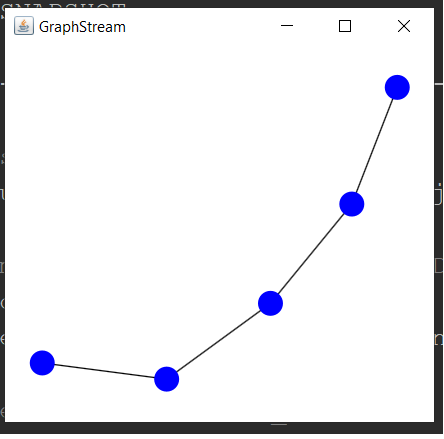
\includegraphics[scale=0.5]{img/graph.png}
        \caption{Árbol AVL tipo grafo}
        \label{fig:imagen}
    \end{figure}

\section{Cuestionario:}
    \begin{enumerate}
        \item \textbf{¿Explique como es el algoritmo que implementó para obtener el factor de equilibrio de un nodo?}.
    \end{enumerate}
El factor de equilibrio para cada nodo fue implementado como atributo dentro de dicha clase, sin embargo, si se deseara hallar dicho factor sin tenerlo como atributo se podría hacer uso de una función recursiva, donde se recibe como parámetro el nodo raiz y compara, si dicho nodo es nulo, eso significa que su altura es 0, por lo cual se retorna 0, si esto no ocurre, se obtiene la altura izquierda y derecha del árbol haciendo llamado dos veces más al método para cada hijo de la raiz, una vez obtenidas las alturas se halla la mayor y se le suma 1, el retorno de este valor contará como sumatoria desde el nodo más alto hasta la raiz principal, devolviendo su altura máxima.

\section{Conclusiones:}
* La implementación de los métodos del árbol AVL nos enseñó la importancia de mantener el balance en las estructuras de datos para optimizar las operaciones de búsqueda, inserción y eliminación.

    - Aprendimos a valorar la eficiencia del árbol AVL en conjuntos de datos grandes, ya que ofrece un tiempo de ejecución garantizado en el peor caso de O(log n), lo que lo hace adecuado para aplicaciones que requieren un acceso rápido y eficiente a los datos.
\clearpage
\section{Referencias}
\begin{itemize}	
        \item \url{https://www.geeksforgeeks.org/introduction-to-avl-tree/}	
        \item \url{https://www.geeksforgeeks.org/insertion-in-an-avl-tree/}
        \item \url{https://www.geeksforgeeks.org/deletion-in-an-avl-tree/}
        \item \url{https://www.javatpoint.com/avl-tree}
        \item \url{https://docs.oracle.com/javase/tutorial/java/generics/types.html}
        \item \url{https://algorithmtutor.com/Data-Structures/Tree/AVL-Trees/}
\end{itemize}
 \end{document}